% Trying to break the document up a bit.  This command simply inserts the contents of the file at this point.  It contains the document license, preamble, and title page: things that aren't likely to change more than once.  This can be used to separate discrete parts of a document into files that are easier to edit at one time.
%%%%%%%%%%%%%%%%%%%%%%%%%%%%%%%%%%%%%%%%%%%%%%%%%%%%%%%%%%%%%%%%%%%%%%
% This layout was adapted from one found at latextemplates.com which
% was adapted from another.
%
% License: CC BY-NC-SA 3.0
% (http://creativecommons.org/licenses/by-nc-sa/3.0/)
%
% Original header:
%
% This is a LaTeX version of the sample laboratory report from
% Virginia Tech's copyrighted 08-09 CHEM 1045/1046 lab manual.
% Reproduction of this one appendix section for academic purposes
% should fall under fair use.
%
%%%%%%%%%%%%%%%%%%%%%%%%%%%%%%%%%%%%%%%%%%%%%%%%%%%%%%%%%%%%%%%%%%%%%%

\documentclass{article}

\usepackage{graphicx}
% \usepackage[acronym]{glossaries} % Lets us use acronyms
\usepackage{multicol}
\usepackage{amsmath}
\usepackage{siunitx} % SI units in math mode
%\usepackage[usenames]{color}
\usepackage{subcaption}

\author{}
\title{ELEC-313 \\ Lab 9: Common-Emitter Transistor Amplifier\\ }
\date{\today}

% \loadglsentries{acronyms} % Actually loads 'acronyms.tex'
% \makeglossaries

\begin{document}

\maketitle

\begin{center}
  \begin{tabular}{lr}
    Date Performed: & November 20, 2013 \\
    Partners:       & Charles Pittman    \\
    & Stephen Wilson     \\
  \end{tabular}
\end{center}

\newpage

%\tableofcontents
%\listoffigures
%\listoftables
%\newpage

% Number the enumerate environment (unordered lists) by letter:
% \renewcommand{\labelenumi}{\alph{enumi}.}

\section{Objective}
\label{sec:objective}

The objective is to construct and observe the operation of a CMOS inverter and NAND gate.

\section{Equipment}
\label{sec:equipment}

\begin{tabular}{ll}
  \centering
  Transistor: 1N4007                          & Power supply: HP E3631A       \\
  Resistors: \SI{330}{\ohm} (x3), \SI{2.2}{\kilo\ohm}, \SI{33}{\kilo\ohm}               & Multimeters: Fluke 8010A (x2),  \\
\end{tabular}

 \section{Schematics}
 \label{sec:schematics}

 \begin{figure}[hbtp]
   \centering
   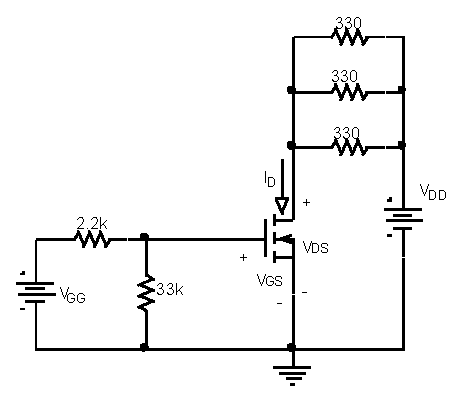
\includegraphics[width=0.6\textwidth]{circuit}
   \caption{\label{fig:circuit} Circuit used in this lab.}
 \end{figure}

 % \begin{figure}[hbtp]
 %   \centering
 %   \begin{subfigure}[b]{0.4\textwidth}
 %     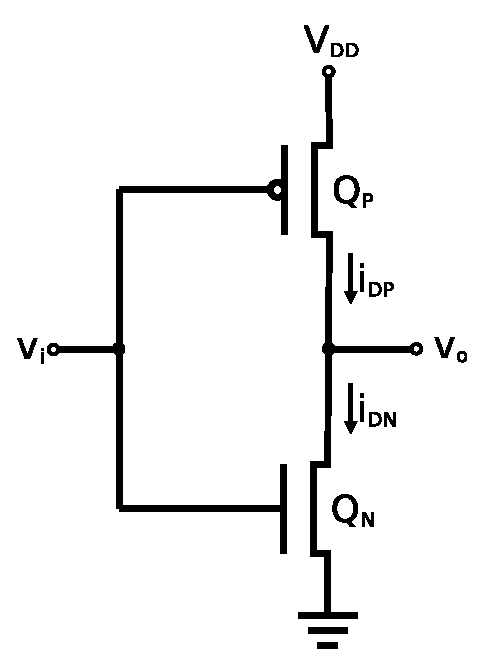
\includegraphics[width=\textwidth]{invert}
 %     \caption{\label{schem:inverter} CMOS Inverter}
 %   \end{subfigure}%
 %   ~
 %   \begin{subfigure}[b]{0.4\textwidth}
 %     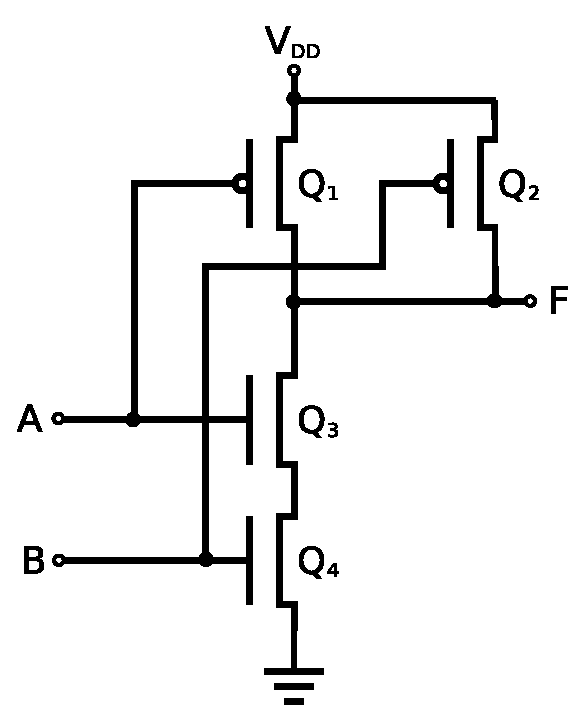
\includegraphics[width=\textwidth]{nand}
 %     \caption{\label{schem:nand} CMOS NAND}
 %   \end{subfigure}
 %   \caption{\label{fig:schematics} Circuits used in this lab.}
 % \end{figure}

\section{Procedure}
\label{sec:procedure}

\subsection{DC Characteristics}
\label{sec:inverter}

\subsection{Small-Signal Transconductance}
\label{sec:nand}

\section{Results}
\label{sec:results}

\begin{figure}[hbtp]
  \centering
  \resizebox{1.0\textwidth}{!}{% GNUPLOT: LaTeX picture with Postscript
\begingroup
  \makeatletter
  \providecommand\color[2][]{%
    \GenericError{(gnuplot) \space\space\space\@spaces}{%
      Package color not loaded in conjunction with
      terminal option `colourtext'%
    }{See the gnuplot documentation for explanation.%
    }{Either use 'blacktext' in gnuplot or load the package
      color.sty in LaTeX.}%
    \renewcommand\color[2][]{}%
  }%
  \providecommand\includegraphics[2][]{%
    \GenericError{(gnuplot) \space\space\space\@spaces}{%
      Package graphicx or graphics not loaded%
    }{See the gnuplot documentation for explanation.%
    }{The gnuplot epslatex terminal needs graphicx.sty or graphics.sty.}%
    \renewcommand\includegraphics[2][]{}%
  }%
  \providecommand\rotatebox[2]{#2}%
  \@ifundefined{ifGPcolor}{%
    \newif\ifGPcolor
    \GPcolortrue
  }{}%
  \@ifundefined{ifGPblacktext}{%
    \newif\ifGPblacktext
    \GPblacktextfalse
  }{}%
  % define a \g@addto@macro without @ in the name:
  \let\gplgaddtomacro\g@addto@macro
  % define empty templates for all commands taking text:
  \gdef\gplbacktext{}%
  \gdef\gplfronttext{}%
  \makeatother
  \ifGPblacktext
    % no textcolor at all
    \def\colorrgb#1{}%
    \def\colorgray#1{}%
  \else
    % gray or color?
    \ifGPcolor
      \def\colorrgb#1{\color[rgb]{#1}}%
      \def\colorgray#1{\color[gray]{#1}}%
      \expandafter\def\csname LTw\endcsname{\color{white}}%
      \expandafter\def\csname LTb\endcsname{\color{black}}%
      \expandafter\def\csname LTa\endcsname{\color{black}}%
      \expandafter\def\csname LT0\endcsname{\color[rgb]{1,0,0}}%
      \expandafter\def\csname LT1\endcsname{\color[rgb]{0,1,0}}%
      \expandafter\def\csname LT2\endcsname{\color[rgb]{0,0,1}}%
      \expandafter\def\csname LT3\endcsname{\color[rgb]{1,0,1}}%
      \expandafter\def\csname LT4\endcsname{\color[rgb]{0,1,1}}%
      \expandafter\def\csname LT5\endcsname{\color[rgb]{1,1,0}}%
      \expandafter\def\csname LT6\endcsname{\color[rgb]{0,0,0}}%
      \expandafter\def\csname LT7\endcsname{\color[rgb]{1,0.3,0}}%
      \expandafter\def\csname LT8\endcsname{\color[rgb]{0.5,0.5,0.5}}%
    \else
      % gray
      \def\colorrgb#1{\color{black}}%
      \def\colorgray#1{\color[gray]{#1}}%
      \expandafter\def\csname LTw\endcsname{\color{white}}%
      \expandafter\def\csname LTb\endcsname{\color{black}}%
      \expandafter\def\csname LTa\endcsname{\color{black}}%
      \expandafter\def\csname LT0\endcsname{\color{black}}%
      \expandafter\def\csname LT1\endcsname{\color{black}}%
      \expandafter\def\csname LT2\endcsname{\color{black}}%
      \expandafter\def\csname LT3\endcsname{\color{black}}%
      \expandafter\def\csname LT4\endcsname{\color{black}}%
      \expandafter\def\csname LT5\endcsname{\color{black}}%
      \expandafter\def\csname LT6\endcsname{\color{black}}%
      \expandafter\def\csname LT7\endcsname{\color{black}}%
      \expandafter\def\csname LT8\endcsname{\color{black}}%
    \fi
  \fi
  \setlength{\unitlength}{0.0500bp}%
  \begin{picture}(7200.00,5040.00)%
    \gplgaddtomacro\gplbacktext{%
      \csname LTb\endcsname%
      \put(946,704){\makebox(0,0)[r]{\strut{}0mA}}%
      \csname LTb\endcsname%
      \put(946,1156){\makebox(0,0)[r]{\strut{}10mA}}%
      \csname LTb\endcsname%
      \put(946,1609){\makebox(0,0)[r]{\strut{}20mA}}%
      \csname LTb\endcsname%
      \put(946,2061){\makebox(0,0)[r]{\strut{}30mA}}%
      \csname LTb\endcsname%
      \put(946,2513){\makebox(0,0)[r]{\strut{}40mA}}%
      \csname LTb\endcsname%
      \put(946,2966){\makebox(0,0)[r]{\strut{}50mA}}%
      \csname LTb\endcsname%
      \put(946,3418){\makebox(0,0)[r]{\strut{}60mA}}%
      \csname LTb\endcsname%
      \put(946,3870){\makebox(0,0)[r]{\strut{}70mA}}%
      \csname LTb\endcsname%
      \put(946,4323){\makebox(0,0)[r]{\strut{}80mA}}%
      \csname LTb\endcsname%
      \put(946,4775){\makebox(0,0)[r]{\strut{}90mA}}%
      \csname LTb\endcsname%
      \put(1078,484){\makebox(0,0){\strut{}0 V}}%
      \csname LTb\endcsname%
      \put(2223,484){\makebox(0,0){\strut{}1 V}}%
      \csname LTb\endcsname%
      \put(3368,484){\makebox(0,0){\strut{}2 V}}%
      \csname LTb\endcsname%
      \put(4513,484){\makebox(0,0){\strut{}3 V}}%
      \csname LTb\endcsname%
      \put(5658,484){\makebox(0,0){\strut{}4 V}}%
      \csname LTb\endcsname%
      \put(6803,484){\makebox(0,0){\strut{}5 V}}%
      \put(176,2739){\rotatebox{-270}{\makebox(0,0){\strut{}$I_D$}}}%
      \put(3940,154){\makebox(0,0){\strut{}$V_{DS}$}}%
    }%
    \gplgaddtomacro\gplfronttext{%
      \csname LTb\endcsname%
      \put(5816,4602){\makebox(0,0)[r]{\strut{}$V_{GS}$ = 2.11}}%
      \csname LTb\endcsname%
      \put(5816,4382){\makebox(0,0)[r]{\strut{}$V_{GS}$ = 2.31}}%
      \csname LTb\endcsname%
      \put(5816,4162){\makebox(0,0)[r]{\strut{}$V_{GS}$ = 2.51}}%
      \csname LTb\endcsname%
      \put(5816,3942){\makebox(0,0)[r]{\strut{}$V_{GS}$ = 2.71}}%
      \csname LTb\endcsname%
      \put(5816,3722){\makebox(0,0)[r]{\strut{}$V_{GS}$ = 2.91}}%
    }%
    \gplbacktext
    \put(0,0){\includegraphics{graph}}%
    \gplfronttext
  \end{picture}%
\endgroup
}
  \caption{\label{fig:graph} Graph}
\end{figure}

\section{Conclusion}
\label{sec:conclusion}

 \section{Equations}
 \label{sec:equations}

% LaTeX sees blank lines as a start of another paragraph.  To avoid
% unnecessary vertical spaces between equations, and still visually
% separate in source, put a comment between them.
%
 \begin{equation}
   \label{eq:transconduct}
   g_m = \frac{I_{D2}-I_{D1}}{V_{GS2}-V_{GS1}}
 \end{equation}
% %
% \begin{equation}
%   \label{eq:ripple}
%   V_r = V_{max} - V_{min}
% \end{equation}

\end{document}
